\subsection{Flujo de efectivo}

El flujo de efectivo permite analizar la capacidad de la empresa para generar recursos suficientes que le permitan cumplir con sus obligaciones, invertir y expandirse.

Para calcular el flujo neto, se consideran tres categorías principales de flujos de caja:

\begin{itemize}
    \item \textbf{Flujo de caja operativo: } Corresponde a los fondos generados por las actividades principales del negocio, ajustados por conceptos como depreciación, amortización, intereses y pago de impuestos.
    \item \textbf{Flujo de caja de inversión: } Incluye los desembolsos destinados a la adquisición de activos, tanto tangibles como intangibles, necesarios para el desarrollo de la empresa.
    \item \textbf{Flujo de caja de financiamiento: } Hace referencia a los recursos obtenidos de inversionistas y a los pagos relacionados con dicho financiamiento.
\end{itemize}

La suma de estos tres tipos de flujos determina el monto total de efectivo generado por la empresa en el periodo evaluado.

\vspace{2mm}
\begin{minipage}{0.8\textwidth}
\centering
\captionof{table}[{Flujo de caja de efectivo }]{ Flujo de caja de efectivo}
\label{flujoOperacional}
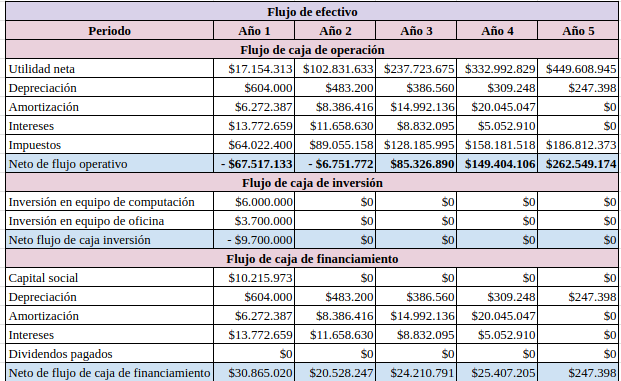
\includegraphics[width=0.9\textwidth]{Content/Images/AF/FlujoDeEfectivo.png}
\footnote{Nota. \textup{Fuente : Autores}}
\end{minipage}
